We evaluate the prototype on a single-host emulation, organized by the four
mechanisms of \S~\ref{sec:architecture} (M1--M2, M3, and M4).
Three
further experiments delimit what \systemname{} does not promise rather than
evaluate a mechanism--a Raft consensus baseline (\S~\ref{sec:eval-raft}), a
CRDT-LWW semantic falsification (\S~\ref{sec:eval-crdt}), and command-to-core
WAN backhaul recovery (\S~\ref{sec:eval-wan}). Finally,
\S~\ref{sec:eval-network} varies the two axes the mechanism cells hold fixed:
connectivity over time, and the number of responder edges.

The propagation, recovery, and
throughput cells use a single responder path, so reported latencies are per-path,
not aggregate. Each cell repeats $n=30$ unless noted, with median and p95
reported. Partitions cut only the targeted path with \textit{tc}, so each cell
isolates one effect.
Impairment uses two \textit{tc-netem} profiles informed by published mesh
measurements~\cite{zimbelman2022mesh,kumbhar2015legacy}.
Table~\ref{tab:evaluation} collects the primary service-path numbers.

\begin{table}[t]
\centering
\caption{Service-path measurements for responder propagation, WAN recovery, command serialization, and responder isolation.}
\label{tab:evaluation}
\scriptsize
\setlength{\tabcolsep}{3pt}
\begin{tabularx}{\columnwidth}{@{}p{0.34\columnwidth}p{0.25\columnwidth}X@{}}
\toprule
\textbf{Path / cell} & \textbf{Result} & \textbf{Interpretation} \\
\midrule
% Auto-generated by scripts/generate_tables.py.
% Do not edit; re-run the script after evaluation JSONL changes.
\textit{Responder-to-command propagation} & & \\
  \hspace{2mm}queue depth = 1 ($n=30$) & median 710.1\,ms; p95 832.1\,ms & outbox-to-command journal path \\
  \hspace{2mm}queue depth = 10 ($n=30$) & median 639.4\,ms; p95 719.5\,ms & outbox-to-command journal path \\
  \hspace{2mm}queue depth = 100 ($n=30$) & median 931.5\,ms; p95 1045.5\,ms & outbox-to-command journal path \\
\addlinespace
\textit{Command-to-core WAN recovery} & & \\
  \hspace{2mm}partition = 1\,s ($n=30$) & median 0.75\,s; p95 0.92\,s & support-path backhaul, not command authority \\
  \hspace{2mm}partition = 10\,s ($n=30$) & median 0.91\,s; p95 1.04\,s & support-path backhaul, not command authority \\
  \hspace{2mm}partition = 60\,s ($n=30$) & median 0.23\,s; p95 1.05\,s & support-path backhaul, not command authority \\
\addlinespace
\textit{Command journal serialization} & & \\
  \hspace{2mm}direct \texttt{/accept} ($n=29$) & median 356.3 events/s; p95 491.7 & sequencer: command accept + journal write only \\
  \hspace{2mm}end-to-end via outbox ($n=29$) & median 159.4 events/s; p95 163.9 & full responder outbox $\rightarrow$ push-batch $\rightarrow$ command path \\
\addlinespace
\textit{Command commit during responder isolation} & & \\
  \hspace{2mm}direct command accept path ($n=20$) & 20/20 commits; seq. 1--20; 0 duplicate seqs. & direct \texttt{/accept/event-batch} path; median/p95 latency 5.76/7.32\,ms \\
\bottomrule

\end{tabularx}
\end{table}

\subsection{Authority boundary and journal sequencing (M1--M2)}
\label{sec:eval-independence}
\label{sec:eval-m1}
\label{sec:eval-m2}

M1--M2 serve R3, and R1 for command-side writes.

With one responder isolated for ten seconds, direct single-event POSTs to
\textit{/accept/event-batch} all commit, assigning consecutive non-duplicate
\textit{event\_seq} values at single-digit millisecond latency
(Table~\ref{tab:evaluation}). Stale or absent \textit{X-Command-Epoch} values are
rejected before journal work. Responder reachability is therefore not in the commit
path.

Saturation throughput at the linearization point (Table~\ref{tab:evaluation})
reflects a single-writer serializer. Even a generous 10 authority-bearing events
per minute is 0.17 events/s, so the measured 356.3 events/s exceeds plausible
incident demand by three orders of magnitude.

\subsection{Durable outbox and idempotent submission (M3)}
\label{sec:eval-m3}

M3 (the durable responder outbox with \textit{client\_event\_id} idempotency)
serves R1 and R2.

Median propagation stays sub-second across queue depths 1--100; the p95 at
depth 100 marginally exceeds 1~s (1045.5~ms, Table~\ref{tab:evaluation}).

Replaying 50 unique \textit{client\_event\_id} values five times each leaves exactly 50
journal rows across $n=30$ runs: forwarding is at-least-once and deduplicated at the
journal, so submission is effectively exactly-once at the linearization point. Across
process restart, 50 outbox submissions survive a responder-Postgres power cycle, then
forward with no duplicates and consecutive \textit{event\_seq}, reaching journal
consistency about 2.6\,s after recovery---the runtime witness for R2.

\subsection{Fenced promotion (M4)}
\label{sec:eval-promotion}
\label{sec:eval-m4}

M4 (fenced promotion with stale-epoch rejection) serves R3 under command transfer and
exercises C2: promotion preserves single authority across an epoch change and rejects
stale-epoch traffic, on the service path, before any incident-journal work.

Protocol cost is single-digit milliseconds across all three phases of a transition
(Figure~\ref{fig:promotion-cost}). Commit phases~$A$ and~$C$ have medians
\promotionMedianA{} and \promotionMedianC{}; the phase~B stale-rejection path is
$2.5\times$ cheaper by construction, since the fence rejects stale traffic before the
journal write. Operator confirmation sits in the critical path by design and dominates
wall-clock; the protocol contribution is orders of magnitude smaller, an operator cost
rather than a network cost.

\begin{figure}[t]
\centering
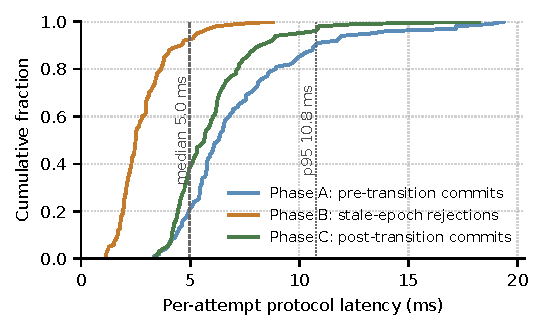
\includegraphics[width=0.85\columnwidth]{figures/fig_promotion_cost.pdf}
\caption{Fenced-promotion protocol cost by phase. Phase~A is pre-transition
commits at epoch~$e$, phase~B is stale-epoch rejections at the journal boundary,
phase~C is post-transition commits at epoch~$e+1$. $n=\promotionN$ events
($\promotionNPerPhase$ per phase). Vertical markers are pooled across phases:
median \promotionMedianCombined{}, p95 \promotionPNinetyFiveCombined{}. The
cost shown is the protocol path only; the operator-confirm step is excluded by
design.}
\label{fig:promotion-cost}
\end{figure}

In five live service-path runs, phase~$A$ commits 20/20 events at epoch~1, phase~$B$
returns 20/20 HTTP~409 rejections for the stale epoch and adds zero
incident-journal rows, and phase~$C$ commits 20/20 events at epoch~2. The incident
journal holds 200 rows total, split 100/100 between epochs, with no
\textit{event\_seq} value appearing under both.

\subsubsection{Two-edge fenced promotion}
\label{sec:eval-two-edge}

The results above hold at one acceptor. We additionally exercise promotion across two
independent vehicle edges, each with its own database, with the incumbent partitioned
from the network. The candidate bootstraps the journal prefix from core, verifies it is
contiguous, obtains the next epoch, and only then takes the role; responders are
repointed at the new command.

Two outcomes matter for R3, and both are measured rather than asserted. First, when the
superseded edge reconnects and forwards the writes it buffered while isolated, core
refuses them because another node holds the epoch; the edge demotes itself, and its own
accept path then refuses authority-bearing writes. Its buffered rows are retained for
reconciliation, and the authoritative journal is unchanged throughout---the fork
is contained at the
journal boundary and never admitted. Second, when the \emph{current} holder
loses only its backhaul, it accepts writes while its lease is valid and refuses them
once the lease lapses, recovering when the link returns. It is never informed that
anything happened; it stops on a timeout it cannot renew, which is the honest form of
the guarantee and the reason the availability cost falls where it does.

We do not report a fencing latency here. The transition is dominated by the
lease window, an operator-chosen parameter rather than a property of the
protocol, and the operator confirmation step already dominates wall-clock
(\S~\ref{sec:eval-promotion}).

Verification and falsification costs are strongly asymmetric. The strict variant passes
all six safety invariants over 38.56\,M distinct states in 13.0\,min, whereas each weak
variant is refuted almost immediately: \textit{SingleAuthority} in 185 states (0.85\,s),
\textit{EpochAuthorityCoupling} in 144 (0.77\,s), and \textit{NoForkedJournal} in 1.0\,k
(0.83\,s). Establishing the property is expensive; refuting the weakened rule is not.

\subsection{Scope Boundaries}

\subsubsection{Raft leadership follows the reachable quorum}
\label{sec:eval-raft}

This tests the R3-relevant mismatch between consensus leadership and operational
command authority. The baseline is the three-voter \textit{hashicorp/raft} cluster in
\textit{baseline-raft/}. Each run hard-cuts the current leader $L_0$ from the other
two voters; the reachable majority elects $L_1$ and accepts writes there
(Table~\ref{tab:raft-comparison}). This is correct Raft
behavior---authority moves to a node that can form a quorum~\cite{ongaro2014raft}---and
it is exactly the mechanism mismatch for R3: Raft has no input by which an operator
can pin the writer to an externally designated command edge.


\begin{table*}[t]
\centering
\caption{Raft consensus baseline. Authority follows the reachable quorum, not an
operator-designated command edge.}
\label{tab:raft-comparison}
\scriptsize
\setlength{\tabcolsep}{3pt}
\begin{tabularx}{\textwidth}{@{}p{0.16\textwidth}p{0.39\textwidth}X@{}}
\toprule
\textbf{Scenario} & \textbf{Measured result} & \textbf{Interpretation} \\
\midrule
% Auto-generated by scripts/generate_raft_table.py.
% Do not edit; re-run the script after Raft evaluation JSONL changes.
Event sequencing sanity & leader batch accepted 1 event, deduplicated 1, last seq. 1; journal count 1 & Confirms the Raft FSM assigns \textit{event\_seq} and enforces \textit{client\_event\_id} idempotency. \\
Leader-minority partition & 12/12 runs elected $L_1 \ne L_0$; 12/12 committed 5 writes at $L_1$; new-leader median 3.08\,s, p95 4.43\,s & $L_0$ writes while isolated, during the election: stall then apply timeout 12/12. Once it has stepped down it instead refuses up front, 12/12, at 0.4\,ms against 269.9\,ms in-window. Authority follows the reachable quorum, not an external command designation. \\
\bottomrule

\end{tabularx}
\end{table*}

\subsubsection{CRDT semantics fail for authority-bearing data}
\label{sec:eval-crdt}

This tests C1: mergeable-by-default replication cannot encode authority for
non-commutative incident decisions. It is a semantic falsification, not a speed
comparison.

The CRDT-LWW baseline is four FastAPI replicas using Hanssen's operation-based
Last-Writer-Wins Element Set~\cite{hanssen2025emergency}. It preserves local
acceptance but loses authority-bearing conflicts: concurrent status updates
converge to the latest timestamp, and a later update resurrects a deleted
element. LWW discards the losing status from materialized state, whereas AAL
preserves both writes in an attributed total order. Ordering and attribution are
R3's service-path scope; semantic rejection is an additional guard disclosed in
\S~\ref{sec:non-claims}.

The baseline is deliberately lightweight and in-memory, converging only through
harness-triggered \textit{full\_sync()}: the test needs the merge rule exercised on
concurrent authority-bearing writes, not storage parity. The asymmetry favors
CRDT where it already performs better, which is the
correct bias for a falsification: if mergeable-by-default semantics cannot encode
authority even under favorable conditions, the semantic argument holds regardless
of infrastructure differences.
Table~\ref{tab:crdt-comparison} keeps measured AAL behavior, model-level AAL
safety, and measured CRDT-LWW semantics separate.

\begin{table*}[t]
\centering
\caption{Semantic comparison with a Hanssen-style CRDT-LWW baseline. The concurrent-edit and delete/update rows use \emph{constructed} conflicts, so their 30/30 outcomes are deterministic by design, not sampled.}
\label{tab:crdt-comparison}
\scriptsize
\setlength{\tabcolsep}{3pt}
\begin{tabularx}{\textwidth}{@{}p{0.16\textwidth}p{0.24\textwidth}p{0.25\textwidth}X@{}}
\toprule
\textbf{Scenario} & \textbf{AAL result} & \textbf{CRDT-LWW result} & \textbf{Interpretation} \\
\midrule
% Auto-generated by scripts/generate_tables.py from eval_crdt_baseline.anon.jsonl.
Field-edit propagation & Attributed order preserved; unimpaired service-path medians in Table~\ref{tab:evaluation} & Impaired: qd=10 stressed/degraded 814.1\,ms/2.54\,s; qd=100 degraded 3.97\,s & Measured under different link conditions, so not a latency comparison; both preserve durable propagation, and CRDT anti-entropy is not an authority boundary. \\
Concurrent status edit & Measured prototype path sequences unique events; semantic rejection is model-level/not implemented in that path & 30/30 LWW runs converge; winner counts contained: 30; median 12.8\,ms & LWW accepts both writes and materializes only the latest value; losing op is only recoverable from the op log. \\
Delete/update race & Measured prototype path has no delete/update semantic guard; limitation disclosed & 30/30 runs resurrect the element; median convergence 12.7\,ms & Matches Hanssen's stated LWW delete-semantics caveat. \\
No-partition throughput & Prototype command-journal commit rate median 356.3 events/s (single writer) & CRDT aggregate local accept rate across three writers median 349.2 events/s & Different units; reports write-availability trade-off, not direct speedup. \\
Post-quiescence convergence (60\,s outage, $n=10$) & Prototype command-to-core support-path recovery median 227.0\,ms after a real \textit{tc} WAN cut ($n=30$) & CRDT all-replica convergence median 45.4\,ms after anti-entropy resumes (no link impairment during the wait) & Comparable in outage duration, not transport mechanism; \systemname{} keeps command-local ordering, CRDT converges once anti-entropy is exchanged. \\
\bottomrule

\end{tabularx}
\end{table*}

\subsubsection{Backhaul recovers within about a second of WAN heal}
\label{sec:eval-wan}

This measures command-to-core forwarding after a WAN heal, with a narrowly
targeted \textit{tc} cut of the command-to-core path only, so the measurement
isolates backhaul flush time (Table~\ref{tab:evaluation}). Recovery is bounded
by the forward poll loop and backlog, not outage length, so
non-monotonic medians across 1, 10, and 60~s outages are expected poll-phase effects.

\subsection{Time-varying connectivity and fleet size}
\label{sec:eval-network}

The measurements above hold connectivity fixed for the duration of a cell and
use a single responder. Neither matches a rescue deployment: vehicle
connectivity alternates between regimes, and incidents involve several
responders at once. This subsection varies each axis in turn.

\subsubsection{Regime transitions, not steady state}
\label{sec:eval-schedule}

A single continuous submission stream runs while the responder-to-command path
walks a schedule of regimes---clear, mesh-stressed, mesh-degraded, isolated,
clear---and every event is attributed to the regime in force when it was
submitted. Impairment is destination-filtered, so only the peer path is
affected and each edge keeps full-speed access to its own database. Ten runs of
the schedule submit 540 events in total.

The result is the durable-outbox property observed \emph{across} a transition
rather than inferred from steady state (Table~\ref{tab:netem-schedule}). Under
every degraded-but-connected regime, delivery within the phase is complete.
Under isolation it is zero: no event reaches the authoritative journal while the
path is down, which is the honest statement of what a single-writer boundary
costs. No event is lost. All 540 reach the journal, all ten runs drain fully,
and the outbox backlog peaks at 13 events before collapsing once the link
returns. Recovery---measured from the instant connectivity is restored until
every event pending at that instant is journal-visible---is sub-second across
all ten runs, with a measurement resolution of about 0.4~s set by the polling
interval and query cost. It is bounded by the forwarder's poll cycle and the
backlog depth, not by how long the outage lasted.

\begin{table}[t]
\centering
\caption{Delivery across a connectivity-regime schedule, $n=10$ runs, 540
events. \emph{Within phase} counts events journaled before that phase ended;
\emph{eventually} counts them after the link returns. The gap between the two
columns in the isolated row is the durable outbox doing its job.}
\label{tab:netem-schedule}
\footnotesize
\setlength{\tabcolsep}{5pt}
\begin{tabular}{@{}lrr@{}}
\toprule
\textbf{Regime} & \textbf{Delivered within phase} & \textbf{Delivered eventually} \\
\midrule
% Auto-generated by scripts/generate_network_tables.py.
% Do not edit; re-run the script after evaluation JSONL changes.
Clear & 1.00 & 1.00 \\
Mesh, stressed & 1.00 & 1.00 \\
Mesh, degraded & 1.00 & 1.00 \\
Isolated & 0.00 & 1.00 \\
Clear (restored) & 1.00 & 1.00 \\
\bottomrule

\end{tabular}
\end{table}

\subsubsection{Fleet size}
\label{sec:eval-fleet}

The second axis is the number of responder edges submitting concurrently.
\S~\ref{sec:eval-m1} argues that a single-writer serializer is adequate because
its saturation rate exceeds plausible incident demand; that argument is only as
good as its behaviour when responders multiply. Fleet sizes of 1, 3, 5 and 10
independent responder edges---each with its own database and outbox---submit
simultaneously, five runs each, 20 events per responder
(Table~\ref{tab:fleet-scaling}).

Delivery is complete at every size: 1900 of 1900 events across the sweep. Journal
throughput rises from 19.5 to 182.5 events/s, a factor of 9.4 for a tenfold
increase in offered load, while propagation latency does not degrade---the p95
at ten edges is below the value at five. The single-writer linearization point
therefore absorbs a ten-edge fleet without becoming the bottleneck, which is the
measured form of the claim \S~\ref{sec:eval-m1} makes.

Two limits are worth stating. The throughput figures are not comparable to the
saturation rate in Table~\ref{tab:evaluation}: a 200-event batch is dominated by
fixed per-event latency, not by serializer capacity, so these numbers are a
lower bound on both. And ten edges is where this single host runs out of memory,
not where \systemname{} runs out of headroom---73 containers share one kernel,
one disk and one bridge. What the sweep establishes is the shape of the curve,
not an absolute ceiling.

\begin{table}[t]
\centering
\caption{Concurrent responder edges against the same command edge, five runs per
size, 20 events per responder. Percentiles are arrival-curve percentiles: the
time by which the journal held that share of the batch.}
\label{tab:fleet-scaling}
\footnotesize
\setlength{\tabcolsep}{4pt}
\begin{tabular}{@{}rrrrr@{}}
\toprule
\textbf{Edges} & \textbf{p50} & \textbf{p95} & \textbf{Events/s} & \textbf{Delivered} \\
\midrule
% Auto-generated by scripts/generate_network_tables.py.
% Do not edit; re-run the script after evaluation JSONL changes.
1 & 1.02\,s & 1.02\,s & 19.5 & 1.00 \\
3 & 606.7\,ms & 963.9\,ms & 62.2 & 1.00 \\
5 & 643.7\,ms & 1.35\,s & 74.2 & 1.00 \\
10 & 728.4\,ms & 1.10\,s & 182.5 & 1.00 \\
\bottomrule

\end{tabular}
\end{table}

Neither experiment is a mobility model. No vehicle positions, path loss or RAN
topology are simulated; the regime durations and impairment parameters are
literature-informed and the transitions are synthetic, which is what makes them
reproducible.

Every cell leaves the authority boundary where \S~\ref{sec:architecture} places
it: no forked journal, no submission lost, no write admitted from a node that
does not hold the epoch. \S~\ref{sec:non-claims} details the non-claims.
